\documentclass{article}
\usepackage[pdftex]{graphicx}
\usepackage{amsmath}
\usepackage{verbatim}
\usepackage{enumerate}
\author{Michael Anderson}
\title{Implementation 1}
\begin{document}
\setlength{\parskip}{1em}
\maketitle\center{CS534}
\center{Prof. Fern}
\flushleft
\newpage

\section{Linear Regression}

For this experiment, I implemented both the batch and stochastic gradient descent algorithms, trained them on the provided training data, and compared their total SSE loss against the test data for various initial guesses of $w$. Although it was not specified in the original problem, I treated the first 3 columns of the given datasets as $x_1, x_2$ and $x_3$, respectively, and the last column as $y$. I used a constant learning rate of $\lambda = 1/N$.

For the batch gradient descent algorithm, I defined convergence as a change of no more than $\epsilon = 10^{-8}$ in each element of $w$. After 275 epochs, $w$ converged to the following vector:

$w$ = [-0.5777, -0.3532, 0.5030, 2.2524]

The stochastic gradient descent algorithm did not converge to the level of strictness defined by my $\epsilon$. After a sufficient number of iterations, it instead oscillated very closely around the value of $w$ given above, to within $10^{-4}$ for each element of $w$. To compare this algorithm to the batch algorithm, I simply ran it for 275 iterations as well.

Following are the semi-log plots of the total SSE loss of both algorithms on the test data, as a function of the epoch number. To test how different initial guesses for $w$ might affect the runtime of each algorithm, I tried w = [0,0,0,0]; w = [1,1,1,1]; w = [5,5,5,5]; w = [10,10,10,10]; and w = [50,50,50,50] respectively. Although different initial guesses for $w$'s affected the shape of the convergence curves, they did not affect the final estimate of $w$ \emph{after} each algorithm converged.

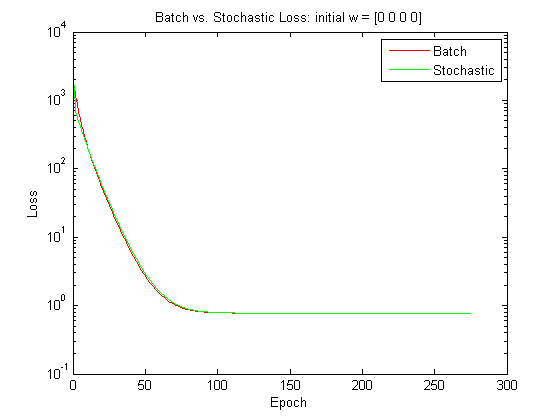
\includegraphics[scale=0.75]{regression_0.png}
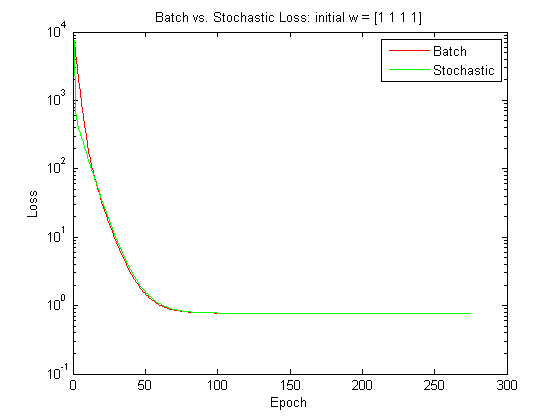
\includegraphics[scale=0.75]{regression_1.png}
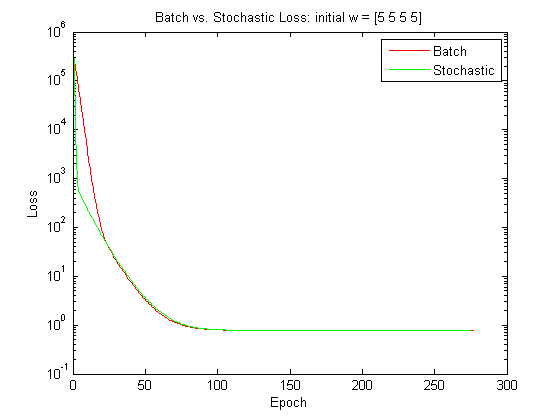
\includegraphics[scale=0.75]{regression_5.png}
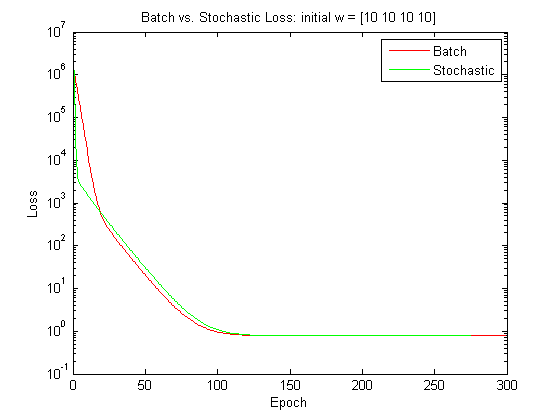
\includegraphics[scale=0.75]{regression_10.png}
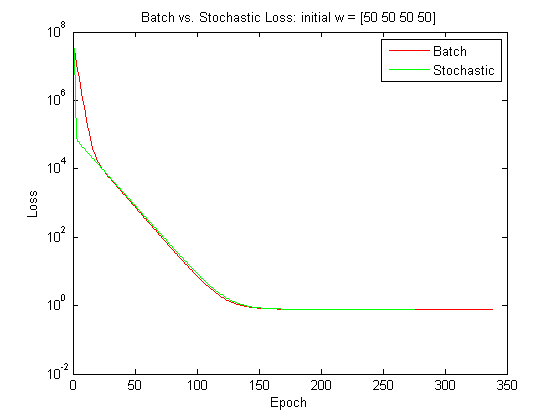
\includegraphics[scale=0.75]{regression_50.png}

There are a number of observations to be made from the above plots. First, as might be expected, when the initial w is far from the true w both the stochastic and batch algorithms take a significantly larger number of epochs to reduce the loss to near 0.

Second, in each case the stochastic algorithm very dramatically reduces the loss in the first few epochs. This effect is particularly pronounced for initial guesses of $w$'s that are far from the true $w$. In each case, after one or two dozen epochs, the batch algorithm catches up and they have nearly identical performance from that epoch forward.

Third, from the point that the batch algorithm catches up to the stochastic algorithm in performance, to around the point that the total loss is in the single-digits, the loss functions look like lines. Since my plots are semi-log, this indicates exponential convergence.

In conclusion, this experiment suggests that stochastic gradient descent outperforms batch gradient descent when the initial guess for $w$ is far from the true $w$, and only a small number of epochs are run. For initial guesses of $w$ that are near to the true $w$, or for experiments where a high degree of accuracy for $w$ is required, they perform almost identically.

\section{Batch Perceptron}

For this experiment, I used the perceptron criterion along with gradient descent to find a decision boundary between two linearly-separable classes of data. I used a constant learning rate of $\lambda = 1$. After 32 epochs, my $w$'s stopped changing completely, and the number of misclassifications as well as the perceptron loss went to zero. My final learned $w$ was:

$w$ = [1.5, -0.6289, -0.5215]

Following is a plot of the number of misclassifications as a function of the number of epochs run so far. 

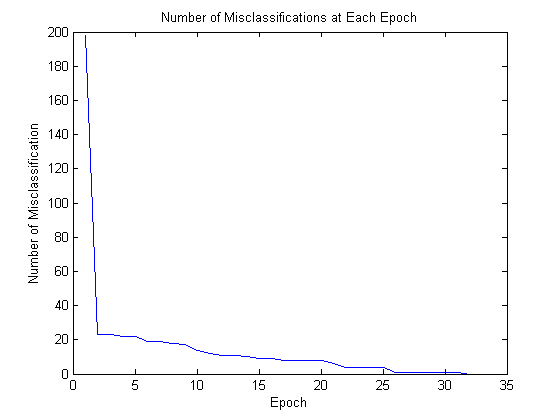
\includegraphics[scale=0.75]{perceptron_progress.png}

Most of the points are correctly classified after the first epoch, and from there the algorithm slowly adjusts itself until it eventually classifies every point correctly. The loss decreases monotonically.

Following is a plot of the data points along with their true class values, as well as my learned decision boundary.

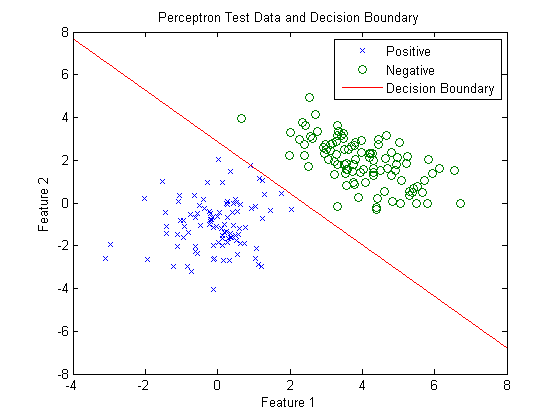
\includegraphics[scale=0.75]{perceptron.png}

It appears in the above plot that one of the +1 class values may be on the wrong side of the decision boundary. To check this, I zoomed in on the plot at this point. As shown in the following plot, the given +1 point is correctly below the decision boundary with the rest of the +1 points.

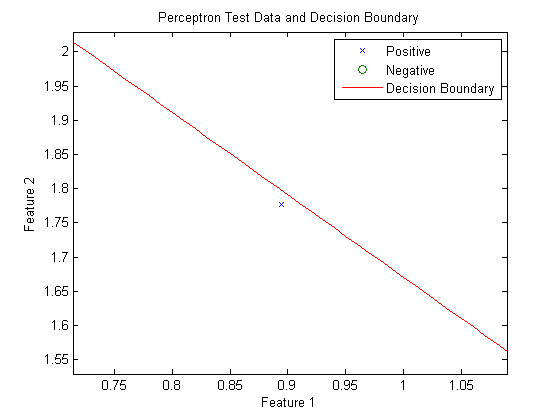
\includegraphics[scale=0.75]{perceptron_zoom.png}

\section{Voted Perceptron}
For this experiment I originally intended to plot the observed loss as a function of time and compare the original voted perceptron algorithm to the algorithm using the $w_{avg}$ trick given in the problem set. Unfortunately, I was blocked by an apparent bug in my code that I was not able to identify, and subsequently my original voted perceptron algorithm did not converge to a reasonable decision boundary. Following is a plot of the given data, along with a decision boundary that shows that my algorithm always seems to predict positive.

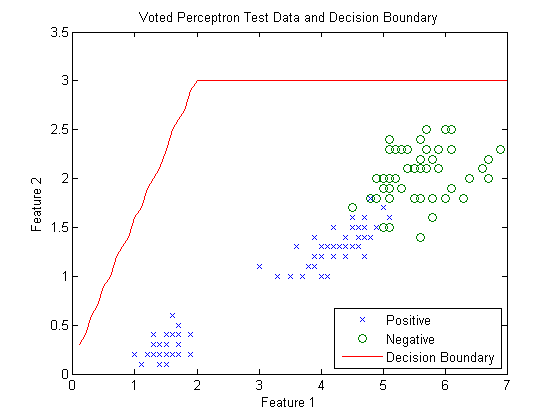
\includegraphics[scale=0.75]{voted_perceptron.png}

\newpage

\section{MATLAB Source Code}

\subsection{Linear Regression}

\begin{verbatim}
% regression.m
% Michael Anderson

% Get training data from file
M = csvread('regression-train.csv');
x_train = M(:,1:3);
n = size(x_train,1);
x_train = cat(2,ones(n,1),x_train);
y_train = M(:,4);
epsilon = 0.0000001*ones(1,4);

% Initialization
w_init = 0;
w_batch = zeros(1,4)+w_init;
w_stochastic = zeros(1,4)+w_init;
iter = 1;
lambda = 1/n;

% Perform batch gradient descent
while true
    cur_w = w_batch(iter,:);
    yhat = x_train*cur_w';
    difs = (yhat-y_train)*ones(1,4);
    gradients = sum(difs .* x_train);
    new_w = cur_w - lambda * gradients;
    
     % Add the new w to the list of w's so far computed
    iter = iter + 1;
    w_batch(iter,:) = new_w;

    % Stop when w stops changing significantly
    if sum(abs(new_w-cur_w) > epsilon) == 0
        break;
    end
end

% Perform stochastic gradient descent
iter = 1;
while true
    % Shuffle the order that the data will be processed in
    perm = randperm(n);
    x_train = x_train(perm, :);
    y_train = y_train(perm, :);

    % Train for one epoch
    cur_w = w_stochastic(iter,:);
    in_epoch_w = cur_w;
    for iter2 = 1:n
        yhat = x_train(iter2,:)*in_epoch_w';
        dif = (yhat-y_train(iter2,:))*ones(1,4);
        gradient = dif .* x_train(iter2,:);
        in_epoch_w = in_epoch_w - lambda * gradient;
    end
    
    % Add the new w to the list of w's so far computed
    iter = iter + 1;
    w_stochastic(iter,:) = in_epoch_w;

    if (iter > 274)
        break;
    end
end

% Get test data from file
N = csvread('regression-test.csv');
x_test = N(:,1:3);
x_test = cat(2,ones(size(x_test,1),1),x_test);
y_test = N(:,4);

% Calculate batch and stochastic loss relative to test data
yhat = x_test*w_batch';
loss_batch = sum((yhat - y_test*(ones(1,size(yhat,2)))).^2);
yhat = x_test*w_stochastic';
loss_stochastic = sum((yhat - y_test*(ones(1,size(yhat,2)))).^2);

% Plot batch and stochastic loss
set(0,'DefaultAxesColorOrder',[1 0 0;0 1 0]);
semilogy(1:size(loss_batch,2), loss_batch, 1:size(loss_stochastic,2), loss_stochastic);
xlabel('Epoch');
ylabel('Loss');
title(sprintf('Batch vs. Stochastic Loss: initial w = [%d %d %d %d]', w_init, w_init,
 w_init, w_init));
legend('Batch', 'Stochastic');
\end{verbatim}
\newpage

\subsection{Batch Perceptron}
\begin{verbatim}
% perceptron.m
% Michael Anderson

% Get data from file
M = csvread('twogaussian.csv');
n = size(M,1);
x = cat(2,ones(n,1),M(:,2:3));
y = M(:,1);

% Initialize
w = [0 0 0];
lambda = 1;
epsilon = 0.00000001 * ones(1,3);

% Perform batch perceptron
for iter = 1:Inf
    delta = [0 0 0];
    misses(iter) = 0;
    for m = 1:n
        u(m) = w * x(m,:)';
        if y(m) * u(m) <= 0;
            delta = delta - y(m) * x(m,:);
            misses(iter) = misses(iter) + 1;
        end
    end
    delta = delta / n;
    w = w - lambda * delta;
    if sum(abs(delta) >= epsilon) == 0
        break;
    end
end

% Plot number of misclassifications as a function of number of epochs
plot(1:iter, misses);
title('Number of Misclassifications at Each Epoch');
xlabel('Epoch');
ylabel('Number of Misclassification');

% Plot data and learned decision boundary. Comment out this block to plot
% misclassifications.
dec_x = -4:0.01:8;
dec_y = -(w(1) + dec_x*w(2))/w(3);
plot(x(1:98,2), x(1:98,3), 'x', x(99:n,2), x(99:n,3), 'o', dec_x,dec_y);
title('Perceptron Test Data and Decision Boundary');
xlabel('Feature 1');
ylabel('Feature 2');
legend('Positive', 'Negative', 'Decision Boundary');
\end{verbatim}
\newpage

\subsection{Voted Perceptron}
\begin{verbatim}
% voted_perceptron.m
% Michael Anderson

% Get data from file
M = csvread('iris-twoclass.csv');
N = size(M,1);
x_orig = cat(2,ones(N,1),M(:,2:3));
y = M(:,1);

% Initialize
w = [0 0 0];
c = 0;
n = 1;

% Perform voted perceptron
for epoch = 1:100
    % Randomly shuffle data at the beginning of each epoch
    ordering = randperm(N);
    x = x_orig(ordering,:);
    y = y(ordering);
    
    for i = 1:N
        u = w(n,:) * x(i,:)';
        if (y(i) * u) <= 0
            w(n+1,:) = w(n,:) + y(i)*x(i,:);
            c(n+1) = 0;
            n = n + 1;
        else
            c(n) = c(n) + 1;
        end
    end
end

% Classify some feature values in a fine grid to determine the decision boundary
for i = 1:1:70
    for j = 0.1:0.1:3
        if sum(c .* ((([1 i/10 j] * w') > 0) * 2 - 1)) < 0
            break;
        end
    end
    dec_y(i) = j;
end

% Plot results
plot(x_orig(1:100,2), x_orig(1:100,3), 'x', x_orig(101:N,2), x_orig(101:N,3), 'o', 
 0.1:0.1:7, dec_y);
title('Voted Perceptron Test Data and Decision Boundary');
xlabel('Feature 1');
ylabel('Feature 2');
legend('Positive', 'Negative', 'Decision Boundary', 'Location', 'SouthEast');

\end{verbatim}

\end{document}